\chapter{Future Work}
In the future, At first,we will study a wider range of paintings and investigate the issues of layer decomposition and stroke segmentation. Different paintings have different stroke patterns. Understanding the rules will improve the success rate of a wider range of paintings. Proper automatic color separation in the overlap regions is not trivial which will also be studied in the future.Second we would try to build high relief based on current algorithm, and based on the depth of high relief , we would try to generate 3D brush painting effects from 2D brush painting, as showed in Figure \ref{Autumn Tree}.
\begin{figure}[H]
	\centering
	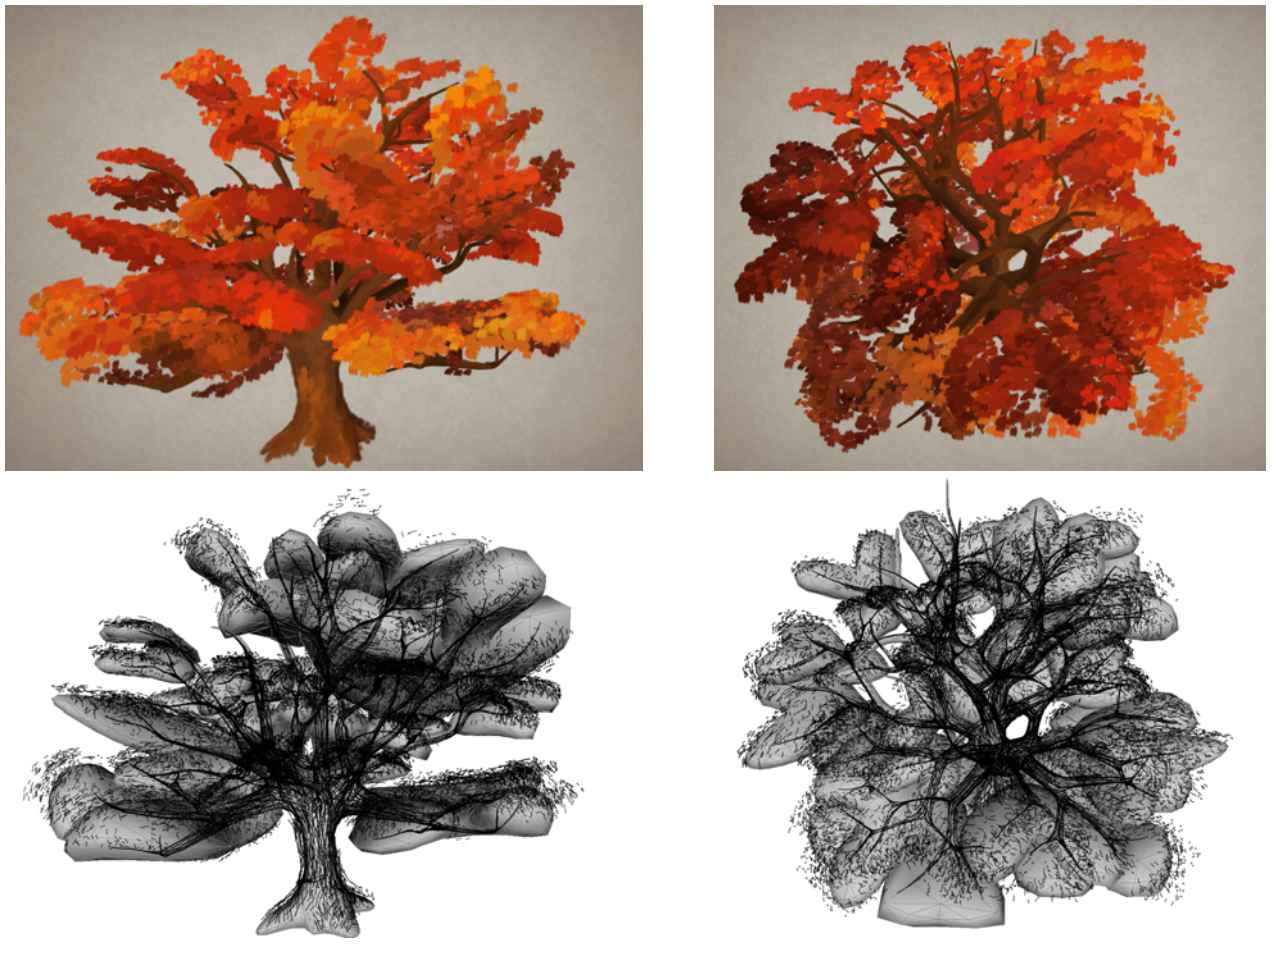
\includegraphics[width=12cm]{autumn_tree.png}
	\caption{3D brush painting : Autumn Tree}
	\label{Autumn Tree}
	\medskip
	The top row shows two different views of a painted tree. The bottom row shows the respective proxy geometry with paint stroke paths on top.
\end{figure}
\section{From 2D Brush Painting to 3D Brush Painting}
\subsection{Abstract} 
With the increasing popularity and development of virtual reality, digital painting on 2D canvases is now being extended to 3D spaces. 3D painting as a new art form are now widely accepted among artists. Software on VR platform such as Tilt Brush and Oculus Quill make 3D painting more and more intuitive for 2D painters.   
We aim to build a system which enable artist to transfer a given 2D brush painting to 3D painting, in a way that gives creative freedom to the artist while maintaining an acceptable level of controllability based on the given 2D brush painting. 

We address this problem into four main steps: 
first, segment strokes from the given 2D brush painting. Since in 3D brush painting, strokes are placed in 3D space based on user input, to mimic such effect, successful strokes segmentation is quite essential. Brush strokes may have high diversity of colour, so layer decomposition may need to be applied. 
Second, stroke refinement, since brush strokes may be over segmented or under segmented, stroke need to be refined. A refinement method based on user input need to be applied. 
Third, transfer 2D strokes to 3D strokes, simulate the effect the 3D stroke with supplied 2D stroke, and 3D volumetric painting would be applied \cite{kim2017canvox}. 
Fourth, 3D strokes placement, based on the layer order and user inputs, we place and blend 3D strokes in 3D space. 

\subsection{Aims and Objectives}
With given 2D brush painting, we aim to design a new approach to generate a 3D brush painting. With such a goal, we need to achieve following:
1. Based on edge and region segmentation, retrieve the reasonable palette colours from input 2D brush painting. 
2. Efficient hierarchical segmentation for brush strokes based on layer decomposition. 
Simulate different scale of brush strokes based on hierarchical segmentation and dynamic branch cutting.
3. Refine stroke segmentation based on user input.
4. Generate correspond 3D brush strokes from 2D brush strokes. 
5. Place and deform 3D brush strokes based on user input.
6. The 3D brush painting must preserve the style and placement order of original 2D brush. 
\subsection{Background and Literature Review:}  

\textbf{ Stroke based rendering:} \newline

The difference between primary space (the 3D world in which objects live) and secondary space (the 2D canvas on which depictions of those objects are created) was highlighted by \cite{schmid2011overcoat}. 

The field of non-photorealistic rendering (NPR) has developed many stylization on 2D canvas. Although traditional photorealistic rendering research focuses on the primary space (e.g., scene representation, visibility determination, global illumination), the NPR community first approached the problem from the opposite direction by focusing entirely on the secondary space of the 2D canvas \cite{hanrahan1990direct}. 

Haeberli’s interactive “Paint By Numbers” system \cite{haeberli1990paint} started the research of stroke based rendering, which proposed a method to fills a 2D canvas with brush strokes when parametric brush stroke are controlled based on given photograph. And similar works which provide automatic approach by placing discrete elements such as paint strokes or stipples to create nonphotorealistic imagery are described stroke-based rendering \cite{hertzmann2003survey} . Interactive stylization of images, video, and animations \cite{lu2010interactive} has also been done.  
These researches mainly focus on how to implement different expressive styles on canvas which algorithmic mapped from primary space. \newline

\textbf{3D painting system:}\newline

The concept of 3D painting system was introduced for more than two decades ago.  Hanrahan \cite{hanrahan1990direct} firstly present a 3D painting system that capable of painting on 3D models, but their work didn’t put transparency and fine detailed painting in consideration. 

From works of  Daily et al. \cite{daily19953d}, 3D painting applied texture map for painting details effect. However, distortion or seams would happen due to 2D parametrization. Meier [1996] first proposed generating brush strokes attached to 3D objects.  Deep Canvas \cite{katanics2003deep}, firstly projected painted strokes on the object’s surface and dynamic 3D camera can be applied which is hard to achieve using traditional 2D paintings. The WYSIWYG NPR system \cite{kalnins2002wysiwyg} focused on algorithmic rendering techniques, which enable artist to achieve silhouette stylization and control hatching directly via a painting interface. Maya Paint Effects (Paint Effects 2011) also projects painted strokes onto the surface of scene geometry and uses them as seed points to create new geometric primitives such as grass or flowers.

\begin{figure}[H]
	\centering
	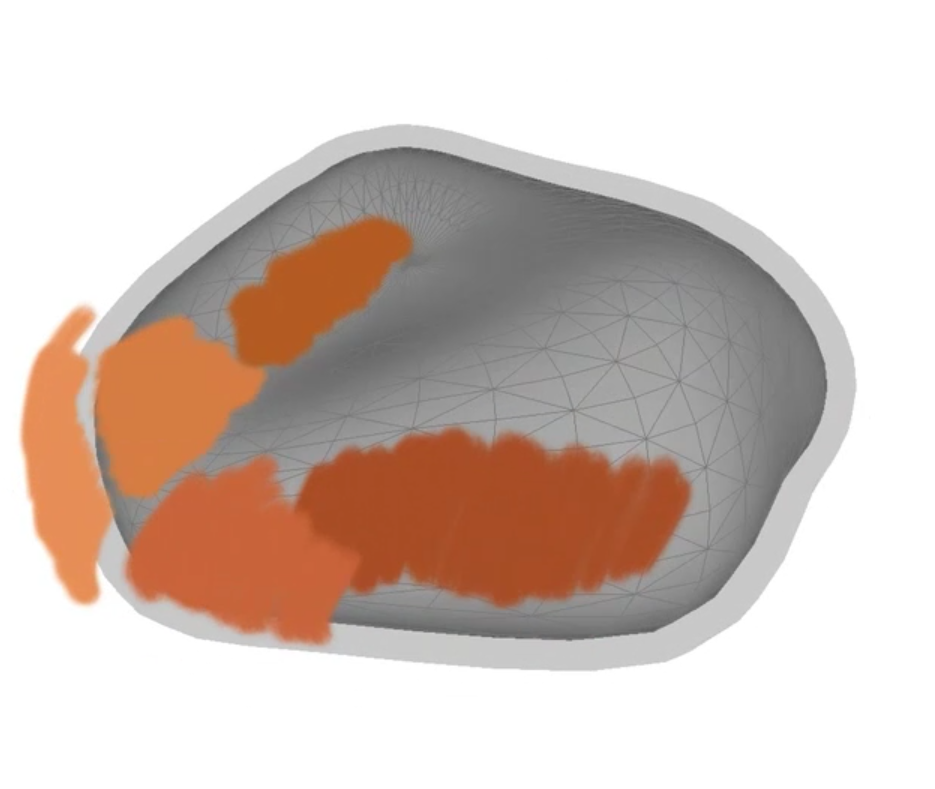
\includegraphics[width=10cm]{level_set.png}
	\caption{3D brush painting on surface level set}
	\label{level set}
\end{figure}

More recently, Overcoat \cite{schmid2011overcoat} introduced an implicit canvas for 3D painting, which enable creating approximate 3D proxy geometry to shape the implicit canvas, it allows us to implement tools for painting along level set surfaces or across different level sets. which means we can project parametric strokes onto the underlying 3D models as showed in Figure \ref{level set}.
These painting systems are focusing on how to paint on surface of known models. In CanvoX \cite{kim2017canvox} extended painting surface to volumetric painting, with GPU-based Octree \cite{lefebvre2005octree}.

With the rapid development of VR systems, it is natural to enable artists to paint in 3D space. In CavePainting \cite{keefe2001cavepainting} firstly create 3D analogy of 2D brush strokes, to create 3D works in a Cave environment. Softwares like Tilt Brush (1) and Quill (2) have recently surged and are now widely accepted by artists to be positioned as a new art form kim's work \cite{kim2017canvox}. For these painting system, quad strips are rendered as painting strokes, which are fully based on user input. 

It is natural to think how to transfer 2D brush paintings to 3D brush painting while preserving its original style. \newline

\textbf{Outline of Proposed Methodology: }\newline

Layer decomposition:  Digital painting with different layers is an integral feature of digital image editing software, such as Photoshop and Sketchbook. Layers offer an intuitive way to edit the colour and geometry of components and localize changes to the desired portion of the final image. Without layers, brush stroke segmentation becomes extremely challenging, since they can overlap and blend with each other. So, at first, we decompose the given 2D brush painting into several layers, which layer contains same colour while each pixel has different transparency. 

Stroke segmentation: As mentioned above, to transfer 2D strokes to 3D strokes, we need to segment each stroke on the painting, inspired by the level set representation of 3D painting in Overcoat, we would segment brush strokes into a hierarchical structure.  

Stroke refinement: To maintain the style of 2D brush painting, successful stroke segmentation is essential for the next step. Wrong segmentation would happen in the process of automatic segmentation, to refine the strokes, user input would be applied. Since the strokes would be a hierarchical structure, hierarchical cut might be applied as well. 

3D stroke analogy: Given segmented strokes, we would create correspond 3D strokes, in which 3D volumetric painting would be applied \cite{kim2017canvox}.

Stroke placement: After generation of 3D stroke analogy for each 2D stroke, a user interface would be supplied for stroke placement.  \newline

\textbf{Proposed timescale for the work:}\newline

Refine the first step of layer decomposition, with the coherent edge of the given 2D brush painting, calculate the palette colour. (4 weeks)

Stroke segmentation into a hierarchical structure, currently, SLIC and hierarchical clustering are in consideration. (4 weeks)

Design the user interface for refine the stroke segmentation. (4 weeks)

3D stroke analogy design. With given segmented strokes, generate corresponding 3D stroke, with detail and style preserved. (6 weeks)

3D stroke placement design. Design the interface for user input, in which 3D strokes can be placed naturally in 3D space while maintaining an acceptable level of controllability. (3 weeks)

Optimization.  (4 weeks)
\newline

\begin{table}[H]
	\centering
	\caption{ Schedule of Future Research Plan}
	\label{my-label}
\begin{tabular}{|l|l|}
	\hline
	\textbf{Research Activity} & \textbf{Target Completion Date} \\ \hline
	\begin{tabular}[c]{@{}l@{}}Design and implement the proposed \\ refinement work. Do experiments accordingly.\end{tabular} & 11/11/2017 \\ \hline
	\begin{tabular}[c]{@{}l@{}}Design the user interface for refine the\\ stroke segmentation.\end{tabular} & 01/2/2018 \\ \hline
	\begin{tabular}[c]{@{}l@{}}3D stroke analogy design and 3D stroke\\ placement design .\end{tabular} & 01/03/2018 \\ \hline
	Optimization. & 01/04/2018 \\ \hline
	Write final Thesis for PhD graduation & 01/06/2018 \\ \hline
\end{tabular}
\end{table}